\documentclass{article}
\usepackage[utf8]{inputenc}
\usepackage{amsmath,amsfonts,amssymb,amsthm,mathtools}
\usepackage{parskip}
\usepackage{color}
\usepackage{booktabs}
\usepackage{hyperref}

\newtheorem{exercise}{Exercise}
\newtheorem{answer}{Answer}

\newcommand{\dd}[2][]{\frac{\partial #1}{\partial #2}}
\newcommand{\dt}[2][]{\frac{d #1}{d #2}}
\newcommand{\dL}{\dt[{\L}]}
\newcommand{\dLi}{\dt[{\Li}]}
\newcommand{\dLmb}{\dt[{\Lmb}]}
\newcommand{\dLfb}{\dt[{\Lfb}]}
\newcommand{\yh}{\hat{y}}

\newcommand{\bracket}[3]{\left#1 #3 \right#2}
\newcommand{\sqb}{\bracket{[}{]}}
\newcommand{\ab}{\bracket{\langle}{\rangle}}
\renewcommand{\b}{\bracket{(}{)}}
\newcommand{\abs}{\bracket{\lvert}{\rvert}}

\newcommand{\0}{\mathbf{0}}
\newcommand{\x}{\mathbf{x}}
\newcommand{\y}{\mathbf{y}}
\newcommand{\f}{\mathbf{f}}
\newcommand{\h}{\mathbf{h}}
\newcommand{\g}{\mathbf{g}}
\newcommand{\mom}{\mathbf{v}}
\newcommand{\F}{\mathbf{F}}
\newcommand{\gfb}{\g_\text{fb}}
\newcommand{\gmb}{\g_\text{mb}}
\newcommand{\gmbt}{\g_{\text{mb}; t}}
\newcommand{\gsmbt}{g_{\text{mb}; t}}
\newcommand{\gsfb}{g_\text{fb}}
\newcommand{\gsmb}{g_\text{mb}}
\newcommand{\gsd}{\g_\text{sd}}
\newcommand{\vh}{\hat{v}}
\newcommand{\mh}{\hat{m}}
\newcommand{\gh}{\mathbf{\hat{g}}}
\newcommand{\gb}{\mathbf{\ab{g}}}
\newcommand{\gssqb}{\ab{g^2}}
\newcommand{\gsb}{\ab{g}}
\newcommand{\bv}{\mathbf{b}}
\newcommand{\ov}{\mathbf{o}}
\renewcommand{\a}{\mathbf{a}}
\newcommand{\X}{\mathbf{X}}
\newcommand{\W}{\mathbf{W}}
\newcommand{\I}{\mathbf{I}}
\renewcommand{\P}{\operatorname{P}\b}

\newcommand{\w}{\mathbf{w}}
\newcommand{\wo}{\w^*}

\renewcommand{\L}{\mathcal{L}}
\newcommand{\Li}{\L_i}
\newcommand{\Lmb}{\L_\text{mb}}
\newcommand{\Lfb}{\L_\text{fb}}
\newcommand{\E}{\operatorname{E}\sqb}
\newcommand{\Var}{\operatorname{Var}\sqb}

\newcommand{\logits}{\ell}
\newcommand{\vlogits}{\boldsymbol{\logits}}
\newcommand{\softmax}{\operatorname{softmax}}
\newcommand{\linear}{\operatorname{linear}}
\newcommand{\relu}{\operatorname{relu}}
\newcommand{\sqerr}{\operatorname{sqerr}}

\newcommand{\func}{\operatorname{func}}
\newcommand{\funcback}{\operatorname{func{.}backward}}
\newcommand{\funcjac}{\operatorname{func{.}jacobian}}
\newcommand{\inputs}{\operatorname{inputs}}
\newcommand{\outputs}{\operatorname{outputs}}

\newcommand{\linearback}{\operatorname{linear{.}backward}}
\newcommand{\reluback}{\operatorname{relu{.}backward}}
\newcommand{\sqerrback}{\operatorname{sqerr{.}backward}}

\newcommand{\linearjac}{\operatorname{linear{.}jacobian}}
\newcommand{\relujac}{\operatorname{relu{.}jacobian}}

\newcommand{\iinmb}{{i \text{ in mb}}}
\newcommand{\mbsize}{M}
\newcommand{\mbavg}{\tfrac{1}{\mbsize} \sum_{\mathclap{\iinmb}}}

\newcommand{\iinfb}{{i \text{ in fb}}}
\newcommand{\fbsize}{N}
\newcommand{\fbavg}{\tfrac{1}{\fbsize} \sum_{i=1}^{\fbsize}}
\newcommand{\lrtrad}{\eta_\text{trad}}
\newcommand{\lravg}{\eta_\text{avg}}

\title{EMAT31530: Practical optimization in AI}
\author{Laurence Aitchison}
\date{}

\begin{document}

\maketitle

Now, we know how PyTorch computes gradients.
However, to practically optimize neural networks, you need a bit more than just gradients: and that's what we'll look at this week!

\section{Minibatching}
So far, we've computed the full gradient based on all the training data in one big batch computation.
In deep learning, this is typically called a ``full batch'' method.
However, remember that GPU memory is very limited, and training datasets are often very, very large.
So full batch training only works in small-scale settings.

As an alternative, we usually use minibatches.
A minibatch is a small subset of the training data (e.g. 128 images out of 60,000 images in the full dataset).
In minibatched training, we calculate the loss, compute the gradients and update the parameters for only the minibatch.

To write down minibatched updates, we need notation for the gradient for the $i$th datapoint,
\begin{align}
  \g_i &= \dLi{\w}.
\end{align}
Here, $\Li$ is the loss for the $i$th datapoint, and $\g_i$ is the gradient for the $i$th datapoint.
We can use the individual datapoint gradient to write down the minibatched gradient. 
The minibatched gradient is just the gradient, averaged over datapoints in the minibatch,
\begin{align}
  \label{eq:gmb}
  \gmb &= \mbavg \g_i =  \mbavg \dLi{\w}.
\end{align}
Here, $\mbsize$ is the minibatch size, and ``$\iinmb$'' gives the set of indicies of datapoints in the current minibatch.
However, it is quite awkward to use this expression directly in PyTorch, as, taken literally, it seems to involve backpropagating through $M$ single-datapoint losses, $\Li$.
In contrast, PyTorch only allows us to (easily) work with a single loss.
We therefore need to define a minibatched loss.
Note that we again use an \textit{average}, rather than a sum, as it makes the code + maths slightly easier.
\begin{align}
  \Lmb &= \mbavg \L_i.
\end{align}
Using PyTorch to differentiate the minibatch loss gives the minibatched gradient, $\gmb$,
\begin{align}
  \dLmb{\w} &= \dt{\w} \b{\mbavg \L_i} = \mbavg \dLi{\w} = \mbavg \g_i = \gmb.
\end{align}
The simplest optimizer that uses minibatching is called ``stochastic gradient descent'', commonly abbreviated to SGD.
This is very similar to gradient descent that we've seen previously, but it uses minibatched gradients, rather than the full batch gradient,
\begin{align}
  \w_{t+1} &= \w_t - \eta \gmbt,
\end{align}
where $\gmbt$ is the minibatched gradient at time $t$.
Note that the ``stochastic'' in SGD refers to the stochasticity induced by randomness in the choice of minibatches.

This additional stochasticity raises a question: what theory do we have to say that SGD still ``works''?
And what do we even mean by ``works'' in this context?
Well, a pretty important feature of an algorithm is whether it eventually converges to the minimum of the loss.
That will (assuming there are no instabilities) happen for e.g.\ SGD applied in the full-batch setting with a fixed learning rate.
However, if you use a fixed learning rate, SGD will get close to the optimum, but won't actually exactly converge to exactly the optimum. 
Instead, it bounce around the optimum forever due to the ``noisy'' minibatched gradient estimates.

However, it turns out we can prove convergence in a slightly modified setting: as the learning rate, $\eta$, decays towards.
Specifically, we can show that if you reduce the learning rate $\eta$, and at the same time, consider an increasing number number of iterations, $T(\eta) = 1/\eta$, then you expect the SGD updates to move the parameters to the same place, but with decreasing variance (the variance is induced by stochasticity in the choice of minibatches). 
Reducing the learning rate as we increase the number of timesteps in effect implies we are averaging over more samples of the minibatch noise.

We start by proving that the expected minibatched update is the same as the full-batch update.
Specifically, we're going to write the full batch loss again as an average,
\begin{align}
  \Lfb &= \fbavg \Li.
\end{align}
where $N$ is the number of datapoints in the full dataset.
The full batch gradient, $\gfb$ is again the average of individual datapoint gradients,
\begin{align}
  \gfb &= \dLfb{\w} = \fbavg \dLi{\w} = \fbavg \g_i.
\end{align}
Now, we can think of the individual datapoint gradient as a random variable, which is equally likely to be the gradient corresponding to any individual datapoint,
\begin{align}
  \P{\gsd} &= \fbavg \delta(\gsd - \g_i)
\end{align}
Critically, this random variable has the right expectation,
\begin{align}
  \E{\gsd} &= \fbavg \g_i = \gfb.
\end{align}
And as the minibatched gradient is just the average of a bunch of independent realisations of $\gsd$ (Eq.~\ref{eq:gmb}),
\begin{align}
  \E{\gmb} &= \gfb,
\end{align}
it also has the right expectation.

Thus, we interpreted the single-datapoint, $\gsd$, or minibatched, $\gmb$, gradients as random variables, and proved that they have the right expectation, $\gfb$.
A statistician would say that $\gsd$ and $\gmb$ are ``unbiased estimators'' of $\gfb$, because $\E{\gsd} = \gfb$ and $\E{\gmb} = \gfb$.
Now, to get a really good estimate of the true-batch gradient, $\gfb$, all we need to do is to average over many independent realisations of $\gsb$ or $\gmb$.
And it turns out we can do this implicitly by considering shrinking the learning rate as we increase the number of timesteps.
Specifically, we consider a number of timesteps that is inversely proportional to the learning rate,
\begin{align}
  \label{eq:T(eta)}  
  T(\eta) = \tfrac{1}{\eta}.
\end{align}
Note that we make sure to choose values of $\eta$ that give integer numbers of steps $T(\eta)$.
The overall change in the parameter, $w$ is,
\begin{align}
  \Delta w &= \eta \sum_{t=1}^{T(\eta)} \gsmbt.
\end{align}
Writing $\eta = 1/T(\eta)$,
\begin{align}
  \Delta w &= \frac{1}{T(\eta)} \sum_{t=1}^{T(\eta)} \gsmbt
\end{align}
Thus, $\Delta w$ is just the average of $T(\eta)$ independent realisations of the minibatched gradient, $\gsmbt$.
Assuming that we consider small changes in $w$, such that the expected gradient doesn't change much across the small part of the trajectory considered (i.e.\ $\E{\gsmbt} = \gsfb$, where $\gsfb$ doesn't change over timesteps), the expected change in weights becomes,
\begin{align}
  \E{\Delta w} &= \frac{1}{T(\eta)} \sum_{t=1}^{T(\eta)} \E{\gsmbt} = \frac{1}{T(\eta)} \sum_{t=1}^{T(\eta)} \gsfb = \gsfb,
\end{align}
which is just the full-batch gradient.
Moreover, as $\Delta w$ is the average of $T(\eta)$ independent realisations of the minibatch gradient, $\gsmbt$, the variance of $\Delta w$ is proportional to $1/T(\eta)$, or to $\eta$ (Eq.~\ref{eq:T(eta)}),
\begin{align}
  \Var{\Delta w} &= \tfrac{1}{T(\eta)} \Var{\gsmb(t)} = \eta \Var{\gsmb(t)},
\end{align}
Thus, as $\eta \rightarrow 0$, the variance in the change in weights $\Var{\Delta w}$ also goes to zero.
%
%such that the expected change in the parameter is the same,
%\begin{align}
%  \E{\Delta w} &= \E{\eta \sum_{t=1}^{T(\eta)} \gsmb(t)}\\
%  \intertext{As $\E{a (X + Y)} = a (\E{X} + \E{Y})$, where $X$ and $Y$ are random variables, and $a$ is a scalar,}
%  \E{\Delta w} &= \eta \sum_{t=1}^{T(\eta)} \E{\gsmb(t)}\\
%  \intertext{As $\E{\gsmb(t)} = \gsfb$ (and we assume that the full batch gradient doesn't change much over the short period we're considering,}
%  \E{\Delta w} &= \eta \sum_{t=1}^{T(\eta)} \gsfb
%  = \eta T(\eta) \gsfb
%  = \eta \tfrac{1}{\eta} \gsfb
%  = \gsfb.
%\end{align}
%Now, lets consider the variance.
%\begin{align}
%  \Var{\Delta w} &= \Var{\eta \sum_{t=1}^{T(\eta)} \gsmb(t)}\\
%  \intertext{As $\Var{a (X + Y)} = a^2 (\Var{X} + \Var{Y})$, where $X$ and $Y$ are independent random variables, and $a$ is a scalar,}
%  \Var{\Delta w} &= \eta^2 T(\eta) \Var{\gsmb(t)}
%  = \eta^2 \tfrac{1}{\eta} \Var{\gsmb(t)}
%  = \eta \Var{\gsmb(t)}.
%\end{align}

Theory is great, but deep learning is a practical subject, so there's a few points of ``wisdom'' and/or common practice. Specifically:
\begin{itemize}
  \item Each pass through the full training dataset is called an ``epoch''.  Deep learning training progress is typically measured in epochs.  Each epoch is composed of many minibatches (minibatches per epoch = dataset size / minibatch size).
  \item Within each epoch, it works slightly better to randomise exactly which datapoints are part of each minibatch, rather than going through the same fixed set of minibatches at each epoch again and again (that's what \verb|shuffle=True| does).
\end{itemize}

\section{The problem with NN optimization}

The simple form of SGD described above doesn't work well, and is rarely used in practice.
The problem all comes down to the interactions between the size of gradients and the learning rates.
Specifically:
\begin{itemize}
  \item If all the gradients are small, then we'd like to use large learning rates to converge reasonably quickly.
  \item If all the gradients are large, then we'd like to use small learning rates to avoid instability.
\end{itemize}
The problem is in practice, gradients in some directions are large, and gradients in some directions are small.
That sets up a conflict: for directions with a large gradient, you'd like to use a small learning rate (to avoid instability).
But for directions with a small gradient, you'd like to use a large learning rate (to converge reasonably quickly).

In practice, real problems have some small and some large gradients.
In that case, you're forced to use a low learning rate (to avoid instability along directions with large gradients), which implies slow convergence along directions with small gradients.
It is this problem that all the optimization tricks discussed below are trying to address.

\section{Momentum}

Momentum is one way to mitigate these issues, as it stabilises learning with large-ish learning rates along high gradient directions.
That allows you to push up the learning rate a bit, allowing faster convergence in the small-gradient directions.
Specifically, the instabilities often look like the diagram below,
\begin{center}
  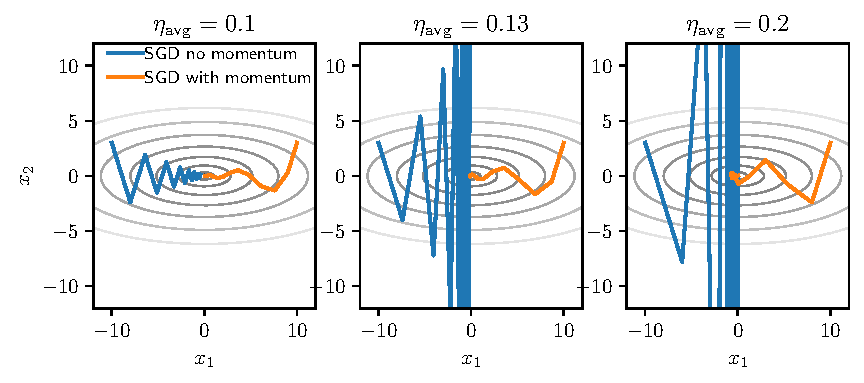
\includegraphics[width=\textwidth]{momentum.pdf}
\end{center}
SGD with no momentum is plotted in the blue lines.
If the learning rate is large, SGD with no momentum can oscillate: at each step, it jumps over the ``horizontal'' in these diagrams.
That's okay if the oscillations decay (i.e.\ left plot below with $\eta=0.1$), in which case you will still converge.
But as the learning rate increases, the oscillations grow, and the learning process diverges (middle and right plots).
Momentum (orange line) allows you to increase learning rates a bit while avoiding this instability.

How does momentum work?
One inuition for momentum (and the origin of the term ``momentum'') is the analogy with Physics.
Specifically, consider a ball rolling around on a hilly landscape, with friction. 
The objective, $\L(\w)$ describes the height of the landscape at any location, $\w$.
``Gravity'' pushes the ball downhill with a force given by the gradient
\begin{align}
  \F(\w) &= - \lrtrad \gfb.
\end{align}
(Note that I'm using two slightly different versions of the momentum update, with two slightly different learning rates: a traditional formaulation with learning rate, $\lrtrad$, that you'll find on the internet, and an ``average'' formulation with learning rate $\lravg$ that makes the effect of momenutum and the connection to later methods such as Adam far clearer).
Taking the mass and gravitational acceleration to be $1$ for simplicity, the equations of motion are,
\begin{subequations}
\begin{align}
  \dt[\mom]{t} &= - (1-\mu) \mom + \F(\w) = - (1-\mu) \mom - \lrtrad \gfb\\
  \dt[\w]{t} &= \mom.
\end{align}
\end{subequations}
Here, the $- (1-\mu) \mom$ term in the first equation represents friction ($\mu$ is between $0$ and $1$).
Discretising these equations with a timestep of $1$ and using the minibatched gradient, $\gmbt$ in place of the full batch gradient, $\gfb$, gives
%\begin{subequations}
%\begin{align}
%  \Delta \mom_t &= -(1-\mu) \mom_t - \lrtrad \gmbt\\
%  \Delta \w_t &= \mom_t
%\end{align}
%\end{subequations}
%which are the traditional momentum updates.
%Here, we use $\Delta \mom_t$ and $\Delta \w_t$ to mean the update in $\mom_t$ and $\w_t$ at this timestep,
%\begin{align}
%  \Delta \mom_t &= \mom_{t+1} - \mom_t & 
%  \Delta \w_t &= \w_{t+1} - \w_t.
%\end{align}
%Thus, the updates can also be written in a slightly simpler form,
\begin{subequations}
\begin{align}
  \label{eq:sgdm:trad:mom}
  \mom_{t+1} &= \mom_t + \dt[\mom]{t} = \mu \mom_t - \lrtrad \gmbt\\
  \label{eq:sgdm:trad:w}
  \w_{t+1} &= \w_t + \dt[\w]{t} = \w_{t} + \mom_{t+1}.
\end{align}
\end{subequations}
This is the traditional parametrisation e.g.\ used in PyTorch (\href{https://pytorch.org/docs/stable/generated/torch.optim.SGD.html}{SGD docs}). Typically we use a momentum of $\mu=0.9$, while the learning rate, $\lrtrad$, needs extensive tuning.

However, I'm really not a fan of the traditional parameterisation: it doesn't help us to understand what's really going on, and conflicts with how other learning rules such as Adam are written down.
These other learning rules use an exponential moving average gradient,
\begin{align}
  \label{eq:gb}
  \gb_{t+1} &= \beta_1 \gb_{t} + (1-\beta_1) \gmbt
\end{align}
This looks alot the ``velocity'' updates in Eq.~\eqref{eq:sgdm:trad:mom}, in that they both have an exponentially decay, with an additive term that depends on the minibatch gradient (the exponential decay is for $\mom$ in Eq.~\eqref{eq:sgdm:trad:mom} and for $\gb$ in Eq.~\eqref{eq:gb}).
However, this form is much easier to interpret, as it is an exponential moving average of minibatch gradients that just estimates the full batch gradient (see exercises for details).
That's why we denote this quantity $\gb_t$ (angle brackets are often used to denote some type of average).
%Specifically, if we are in a region where the underlying gradient doesn't change much,
%\begin{align}
%  \E{\gb_{t}} &= \gfb
%\end{align}
Now, we can write an alternative set of momentum updates,
\begin{subequations}
\begin{align}
  \label{eq:sgdm:avg:g}
  \gb_{t+1} &= \beta_1 \gb_t + (1-\beta_1) \gmbt\\
  \label{eq:sgdm:avg:w}
  \w_{t+1} &= \w_{t} - \lravg \gb_{t+1}
\end{align}
\end{subequations}
This is alot more similar to traditional SGD, in that the parameter updates are again just a learning rate times an estimate of the gradient.
In SGD, we just use a single minibatched gradient estimate, while here, we use an exponential-moving-average over previous minibatch gradient estimates.

This notion of the exponential-moving-averaging gradients allows us to understand why momentum stabilises learning by suppressing oscillations.
Specifically, what happens if we do an exponential moving average over gradients that alternate sign?
Well, the positive and negative terms in that exponential moving average are going to partially cancel, leading to an average gradient that's much smaller in magnitude in these oscillating directions.
And that much smaller gradient implies smaller updates and improved stability.

Now, the existence of these two parameterisations raises the question of how they interrelate.
Specifically, we want to find relationships between $\mu$ and $\lrtrad$ in the traditional formulation and $\beta_1$ and $\lravg$ in the average formulation such that the traditional and average formulations give exactly the same parameter updates at all timesteps.
Specifically, we need the parameter update from the traditional formulation (Eq.~\ref{eq:sgdm:trad:w}) to equal to the update from the alternative formulation (Eq.~\ref{eq:sgdm:avg:w}) at timestep $t$ and $t+1$,
\begin{subequations}
\begin{align}
  \label{eq:prop:t}
  \mom_{t} &= - \lravg \gb_{t} \\
  \label{eq:prop:t+1}
  \mom_{t+1} &= - \lravg \gb_{t+1}.
\end{align}
\end{subequations}
This indicates that we need the momentum in the traditional formulation to be directly proportional to the average gradient.
To achieve that, lets substitute the updates for $\mom_{t+1}$ (Eq.~\ref{eq:sgdm:trad:mom}) and for $\gb_{t+1}$ (Eq.~\ref{eq:sgdm:avg:g}) into Eq.~\eqref{eq:prop:t+1},
\begin{align}
  \nonumber
  \mu \mom_t - \lrtrad \gmbt &= - \lravg \b{\beta_1 \gb_t + (1-\beta_1) \gmbt} \\
  &= - \lravg \beta_1 \gb_t - \lravg (1-\beta_1) \gmbt.
\end{align}
Now, lets use (Eq.~\ref{eq:prop:t}) to substitute for $\mom_t$ on the LHS,
\begin{align}
  - \mu \lravg \gb_{t} - \lrtrad \gmbt &= - \lravg \beta_1 \gb_t - \lravg (1-\beta_1) \gmbt.
\end{align}
Now, the minibatch gradient, $\gmbt$ is a random variable that could (in principle) be anything, and is not e.g.\ deterministically tied to $\gb_t$.
Thus, we're going to consider the equality of the terms proportional to the minibatch gradient, and the terms proportional to $\gb_t$ separately.
For the terms proportional to $\gb_t$ to be equal, we need,
\begin{align}
  - \mu \lravg \gb_{t} &= - \lravg \beta_1 \gb_t.
\end{align}
Thus,
\begin{align}
  \mu &= \beta_1.
\end{align}
And for the terms proportional to $\gmbt$ to be equal,
\begin{align}
  - \lrtrad \gmbt &= - \lravg (1-\beta_1) \gmbt.
\end{align}
Thus,
\begin{align}
  \lrtrad &= \lravg (1-\beta_1) & 
  \lravg &= \tfrac{1}{1 -\beta_1} \lrtrad.
\end{align}
That means if we increase momentum (typically we use $\mu=\beta_1=0.9$) while keeping the traditional momentum, $\lrtrad$, the same, then we are in effect increasing the learning rate, $\lravg$.

\section{RMSProp}

If you remember, the original problem we were solving with momentum was that there are big gradients in some directions, and small gradients in other directions.
You ideally want a big learning rate in directions with a small gradient, to converge quickly.
At the same time, you want a small learning rate in directions with a big gradient, to avoid instability.
Momentum mitigated the problem, by stabilising along high-gradient directions.
But it is also possible to just directly reduce the gradients in the high-gradient directions.
And that's just what RMSProp gives you!
Specifically, RMSProp computes an exponential moving average of the squared gradient, $\gsmbt^2$ then uses the root-mean-square-average gradient to normalize (or adapt) the learning rate,
\begin{align}
  \gssqb_{t+1} &= \beta_2 \gssqb_{t} + (1-\beta_2) \gsmbt^2\\
  %\vh_{t+1} &= \frac{\gsmbt^2}{1-(\beta_2)^t}\\
  \label{eq:rmsprop:w}
  w_{t+1} &= w_t + \frac{\eta}{\sqrt{\gssqb_{t+1}} + \epsilon}\gsmbt.
\end{align}
Note that $\epsilon$ is a small positive constant (usually set to $10^{-8}$) which ensures that we never divide-by-zero.

To understand how RMS prop functions, we assume that we're in a small region, where the gradient is always the same, $\gsmbt = \gsfb$, and if we're in this region for long enough, $\gssqb_{t+1} = \gsfb^2$. 
Now, the weight update is,
\begin{align}
  w_{t+1} &= w_t + \eta \frac{\gsfb}{\sqrt{\gsfb^2} + \epsilon} 
  \intertext{And $\sqrt{\gsfb^2} = \abs{\gsfb}$,}
  w_{t+1} &= w_t + \eta \frac{\gsfb}{\abs{\gsfb} + \epsilon}
  \intertext{Setting $\epsilon = 0$ for simplicity,}
  w_{t+1} &= w_t + \eta \; \text{sign}(\gsfb) \\
  \text{sign}(x) &= \begin{cases}
     1 &\text{if } 0 < x\\
     0 &\text{if } 0 = x\\
    -1 &\text{if } 0 > x
  \end{cases}
\end{align}
So the magnitude of the updates is always around $\eta$, no matter how big the gradients are.
This turns out to be super-important (but not widely understood) intuition for setting $\eta$ to sensible values and for setting up your model to work well with Adam/RMSProp.

\section{Adam}

In practice, RMSProp is rarely, if ever used.
Instead, Adam is perhaps the most common optimizer in deep learning.
Critically, Adam is just RMSProp + Momentum + Bias correction.
Note that the name ``Adam'' breaks down as ``Ada-m'', with the ``Ada'' for ``adaptive'' learning rates, and the ``m'' for momentum.
To combine RMSProp with momentum, we just replace the gradient, $\gsmbt$, in Eq.~\eqref{eq:rmsprop:w} with the exponential moving average gradient, 
\begin{align}
  \gsb_{t+1} &= \beta_1 \gsb_{t} + (1-\beta_1) \gsmbt\\
  \gssqb_{t+1} &= \beta_2 \gssqb_{t} + (1-\beta_2) \gsmbt^2\\
  w_{t+1} &= w_t + \frac{\eta}{\sqrt{\gssqb_{t+1}} + \epsilon}\gsmbt.
\end{align}
These equations show Adam updates without debiasing.
However, there's a problem with these updates: specifically, $\gssqb_{t+1}$ is too small for about the first $1000$ timesteps.
In particular, we typically use a long timescale for the exponential moving average for $\gssqb_{t+1}$: the default is $\beta_2 = 0.999$, which implies a timescale of about $1000$ timesteps.
Moreover, in the absence of any better information, we initialize $\gssqb_0 = 0$.
Combining all this, we have $1-\beta_2 = \tfrac{1}{1000}$, so
\begin{align}
  \gssqb_1 &= \tfrac{1}{1000} g_{\text{mb}; t=1}^2,
\end{align}
thus the first estimate of $\gssqb$ is about 1000 times too small.
Over about 1000 timesteps, $\gssqb$ will converge to more sensible values.
But it still will have spent a long time with a value that is too high.
To fix this issue, the full Adam updates do bias correction:
\begin{align}
  \gsb_{t+1} &= \beta_1 \gsb_{t} + (1-\beta_1) \gsmbt\\
  \gssqb_{t+1} &= \beta_2 \gssqb_{t} + (1-\beta_2) \gsmbt^2\\
  \mh_{t+1} &= \frac{\gssqb_{t+1}}{1-(\beta_1)^t}\\
  \vh_{t+1} &= \frac{\gsb_{t+1}}{1-(\beta_2)^t}\\
  w_{t+1} &= w_t + \frac{\eta}{\sqrt{\vh_{t+1}} + \epsilon}\mh_{t+1}.
\end{align}
To understand what bias correction is doing, see Exercises.

\section{Gradient clipping}

The key problem inducing instability was that the gradients in some directions were too large.
Clipping is perhaps the simplest way to prevent this problem.
Usually, the clip function is defined as,
\begin{align}
  \text{clip}(x, \text{max}, \text{min}) &= \begin{cases}
    \text{max} & \text{if } \text{max} < x\\
    \text{min} & \text{if } x < \text{min} \\
    x & \text{otherwise}
  \end{cases}
\end{align}
In gradient clipping, we'd apply clip to the gradients, with $\text{min} = -\text{max}$.

Gradient clipping seems to work reasonably well in practice, and is often applied.
However, there is an important health-warning when applying gradient clipping in the context of minibatched optimization.
Remember that a key property that we need for optimization to work (e.g.\ to converge to the right answer) was that the expected minibatch gradient should be equal to the full batch gradient,
\begin{align}
  \E{\gmb} &= \gfb.
\end{align}
The problem is that the expected \textit{clipped} gradient is no longer equal to the full batch gradient,
\begin{align}
  \E{\text{clip}(\gmb, \text{min}, \text{max})} &\neq \gfb,
\end{align}
because $\text{clip}$ is a nonlinear function.
This might not be a problem if it happens rarely, or if it happens increasingly rarely if the model converges.
But it is always worth bearing in mind when using clipping!

\section{Exercises}

\begin{exercise}
  Consider an exponential moving average of random variables $X_{t+1}$,
  \begin{align}
    \label{eq:ex:abX}
    \ab{X}_{t+1} &= \beta \ab{X}_{t} + (1- \beta) X_{t+1}
  \end{align}
  where we initialize at,
  \begin{align}
    \ab{X}_{0} &= 0
  \end{align}
  and the means of all the $X_{t+1}$'s are $\mu$,
  \begin{align}
    \label{eq:ex:EX}
    \E{X_{t+1}} &= \mu.
  \end{align}
  Part 1: What is $\E{\ab{X}_{t+1}}$ after an arbitrary number of timesteps?  

  Part 2: Can I multiply by a time-dependent constant, $c_{t+1}$ to form a ``debiased'' estimate,
  \begin{align}
    d_{t+1} &= c_{t+1} \ab{X}_{t+1} 
  \end{align}
  such that
  \begin{align}
    \E{d_{t+1}} &= \mu.
  \end{align}
\end{exercise}

\begin{answer}
Part 1: We begin by taking the expectation of the update (Eq.~\ref{eq:ex:abX})
\begin{align}
  \E{\ab{X}_{t+1}} &= \beta \E{\ab{X}_{t}} + (1- \beta) \E{X_{t+1}}.\\
  \intertext{Substituting Eq.~\eqref{eq:ex:EX},}
  \E{\ab{X}_{t+1}} &= \beta \E{\ab{X}_{t}} + (1- \beta) \mu.\\
  \intertext{To make the notation slightly ``lighter'', use $a_t = \E{\ab{X}_{t}}$,}
  a_{t+1} &= \beta a_t + (1- \beta) \mu.\\
  \intertext{We also have,}
  a_{t} &= \beta a_{t-1} + (1- \beta) \mu.\\
  a_{t-1} &= \beta a_{t-2} + (1- \beta) \mu.\\
  \intertext{Substituting $a_t$ into $a_{t+1}$,}
  a_{t+1} &= \beta (\beta a_{t-1} + (1- \beta) \mu) + (1- \beta) \mu.\\
  a_{t+1} &= \beta^2 a_{t-1} + (1- \beta) (1 + \beta) \mu
  \intertext{Substituting $a_{t-1}$,}
  a_{t+1} &= \beta^2 (\beta a_{t-2} + (1- \beta) \mu)+ (1- \beta) \mu (1 + \beta)\\
  a_{t+1} &= \beta^3 a_{t-2} + (1- \beta) \mu (1 + \beta + \beta^2).
  \intertext{Repeating until we get to $a_0$,}
  a_{t+1} &= \beta^{t+1} a_0 + (1- \beta) \mu \sum_{\tau=0}^{t}\beta^\tau.
  \intertext{As we initialize at $a_0=0$,}
  a_{t+1} &= (1- \beta) \mu \sum_{\tau=0}^{t}\beta^\tau.
  \intertext{Now, the $\sum_{\tau=0}^{t}\beta^\tau$ term is a geometric series.  You can look geometric series up.  Or we can find the value ourselves.  There's a ``trick'' to the proof for a geometric series, which is to consider,}
  (1-\beta) \sum_{\tau=0}^{t}\beta^\tau &= \sum_{\tau=0}^{t}\beta^\tau - \beta \sum_{\tau=0}^{t}\beta^\tau 
  \intertext{Now we can absorb the $\beta$ into the sum,}
  (1-\beta) \sum_{\tau=0}^{t}\beta^\tau &= \sum_{\tau=0}^{t}\beta^\tau - \sum_{\tau=1}^{t+1}\beta^\tau\\
  \intertext{Now, notice that almost all the terms cancel, except those for $\tau=0$ and $\tau=T+1$,}
  (1-\beta) \sum_{\tau=0}^{t}\beta^\tau &= 1 - \beta^{t+1}.
  \intertext{Substituting this back into our form for $a_{t+1}$ gives,}
  \label{eq:ans:a}
  a_{t+1} &= (1-\beta^{t+1}) \mu 
\end{align}
Of course, assuming that $0<\beta<1$, then as $t+1$ goes to infinity, we have,
\begin{align}
  \lim_{t \rightarrow \infty} \beta^{t+1} &= 0 &
  \lim_{t \rightarrow \infty} a_{t+1} &= \mu
\end{align}
The problem is what happens for smaller numbers of timesteps.

Part 2: Therefore, we can choose,
\begin{align}
  \label{eq:ans:c}
  c_{t+1} &= \frac{1}{1-\beta^{t+1}}
  \intertext{Now, the expectation of our debiased estimator, $d_{t+1}$ becomes,}
  \E{d_{t+1}} &= c_{t+1} \E{\ab{X}_{t+1}}
  \intertext{Substituting $a_{t+1} = \E{\ab{X}_{t+1}}$}
  \E{d_{t+1}} &= c_{t+1} a_{t+1}
  \intertext{Substituting for $c_{t+1}$ from Eq.~\eqref{eq:ans:c} and $a_{t+1}$ from Eq.~\eqref{eq:ans:a},}
  \E{d_{t+1}} &= \frac{1}{1-\beta^{t+1}} (1-\beta^{t+1}) \mu = \mu.
\end{align}
So $d_{t+1}$ has the correct expectation.


\end{answer}

%\subsection{Exponential moving averages}
%The exponential moving average gradient estimator was,
%\begin{align}
%  \gb_{t+1} &= \beta_1 \gb_t + (1-\beta_1) \g_t
%\end{align}
%But in what sense is this an ``exponential moving average''?
%
%We know,
%\begin{align}
%  \gb_{t} &= \beta_1 \gb_{t-1} + (1-\beta_1) \g_{t-1}\\
%  \gb_{t-1} &= \beta_1 \gb_{t-2} + (1-\beta_1) \g_{t-2}\\
%  \gb_{t-2} &= \beta_1 \gb_{t-3} + (1-\beta_1) \g_{t-3}
%\end{align}
%Now, substituting $\gb_t$ into $\gb_{t+1}$,
%\begin{align}
%  \gb_{t+1} &= \beta_1 (\beta_1 \gb_{t-1} + (1-\beta_1) \g_{t-1}) + (1-\beta_1) \g_t\\
%  \gb_{t+1} &= \beta_1^2 \gb_{t-1} + (1-\beta_1) (\g_t + \beta_1 \g_{t-1}).
%\end{align}
%Now, substituting $\gb_{t-1}$ into this expression,
%\begin{align}
%  \gb_{t+1} &= \beta_1^2 (\beta_1 \gb_{t-2} + (1-\beta_1) \g_{t-2}) + (1-\beta_1) (\g_t + \beta_1 \g_{t-1})\\
%  \gb_{t+1} &= \beta_1^3 \gb_{t-2} + (1-\beta_1) (\g_t + \beta_1 \g_{t-1} + \beta^2 \g_{t-2}).
%\end{align}
%If we continued doing this, we'd get,
%\begin{align}
%  \gb_{t+1} &= \beta_1^{t+1} \gb_{1} + (1-\beta_1) \sum_{\tau=0}^{t-1}\beta_1^{\tau} \g_{t-\tau}
%\end{align}
%Additionally, we assume that we initialize $\gb_1 = \0$,
%\begin{align}
%  \gb_{t+1} &= (1-\beta_1) \sum_{\tau=0}^{t-1}\beta_1^{\tau} \g_{t-\tau}
%\end{align}
%This can be interpreted as a weighted average, 
%\begin{align}
%  \gb_{t+1} &= \sum_{\tau=0}^{t-1}w_\tau \g_{t-\tau}
%\end{align}
%with weights,
%\begin{align}
%  w_{\tau} &= (1-\beta_1) \beta_1^{\tau}
%\end{align}
%For this to be an exponential moving average, we need the sum of the weights to be $1$.
%\begin{align}
%  \sum_{\tau=0}^{t-1} w_{\tau} &= (1-\beta_1) \underbrace{\sum_{\tau=0}^{t-1} \beta_1^{\tau}}_{\mathclap{\text{geometric series}}}
%\end{align}
%For geometric series, we know,
%\begin{align}
%  \sum_{k=0}^{n-1} r^k &= \frac{1-r^n}{1-r}
%\end{align}
%(for $0 \leq r < 1$).
%Therefore,
%\begin{align}
%  \sum_{\tau=0}^{t-1} w_{\tau} &= (1-\beta_1) \frac{1-\beta_1^t}{1-\beta_1} = 1-\beta_1^t
%\end{align}
%As $0 \leq \beta_1 < 1$, it will quickly approach $0$ as $t$ gets large. 
%In that case, the sum of weights approaches $1$, and it makes sense to regard Eq.~\eqref{eq:gb} as an exponential weighted average.

\end{document}

